% !TEX root =  ../00_thesis.tex

\section{Prolem Setting}
\label{sec:baloo_intro}

\squarepar{%
  Synchronous Transmissions (\ST) is an increasingly used wireless communication technology for low-power multi-hop networks. Popularized by Glossy~\cite{ferrari2011Glossy} in 2011, it has been proven to be highly reliable and energy efficient, as illustrated by the EWSN Dependability Competition ~\cite{schuss2017Competition}, where all wining solutions were based on \ST~\cite{escobar2018Competition,sommer2016Competition,lim2017Competition, escobar2019RedNodeBus, ma2019DeCoT} in the past four years (2016 to 2019).%
}

A \textsl{\ST primitive} refers to a protocol that efficiently realizes broadcast (\ie any-to-all communication) in bounded time, usually relying on \textsl{flooding}.
Flooding is a communication strategy that realizes broadcast by having all receivers of a packet retransmit this same packet to all their neighbours; the packet is thus ``flooded'' through the whole network. \ST makes flooding energy and time efficient by letting multiple wireless nodes transmit the packet \textsl{synchronously}, hence the name of \textsl{Synchronous Transmissions}. The successful reception of the packet can be achieved if the transmitters are tightly synchronized, thanks to \textsl{constructive interference} and the \textsl{capture effect}~\cite{yuan2013LetTalkTogether}.
The synchronization requirements vary from sub-\us to tens of \us, depending on the platform and modulation scheme~\cite{yuan2013LetTalkTogether}.
 %
%\footnote{Some background on flooding and \ST technology is provided in \cref{sec:baloo_overview}.}.
Such a broadcast primitive simplifies the design of network layer protocols: The underlying multi-hop network can be abstracted as a \textsl{virtual single-hop network} and thus be scheduled like a shared bus~\cite{ferrari2012LWB}.
One may refer to \cref{ch:introduction} for more details on \ST.

Since Glossy~\cite{ferrari2011Glossy}, many flavours of \ST primitives have been proposed to improve performance in terms of reliability, latency, and energy consumption.
To be more resilient to strong interference, Robust Flooding~\cite{lim2017Competition} is a primitive that modifies the RX-TX sequence from the original Glossy, whereas RedFixHop~\cite{escobar2016RedFixHop} uses hardware acknowledgements to minimize the number of retransmissions required.
Instead, some primitives aim to minimize latency for specific traffic patterns.
For example, Chaos~\cite{landsiedel2013Chaos} lets all nodes modify the packet being flooded to quickly aggregate information (\eg the max value of all sensor readings) or efficiently perform all-to-all data sharing to achieve distributed consensus~\cite{alnahas2017a2}.
Codecast~\cite{mohammad2018Codecast} also targets many-to-many exchange for a larger amount of data.
Pando~\cite{du2015Pando} is another primitive focused on high throughput, which uses fountain code and packet pipelining for efficient data dissemination.
Syncast~\cite{mohammad2017Improving} aims to reduce the radio on time required to save energy, while Less is More (LiM)~\cite{zhang2017LiM} is a primitive that reduces energy consumption using learning to avoid unnecessary retransmissions during flooding.

\squarepar{%
  All these primitives share the same drawback: Successful \ST requires low-level control of timers and radio events in order to meet \ST tight synchronization requirements (the order of \us).
  This degree of accuracy is difficult to achieve as it requires a detailed knowledge of the underlying hardware, low-level control of the radio operations, and a very careful management of software delays.%
}

As a result, designing a network stack based on \ST is a complex and time consuming task, for which only few solutions have been proposed.
One of the first was the Low-power Wireless Bus (LWB) ~\cite{ferrari2012LWB}, which tries to flexibly support all kinds of traffic patterns in a balanced trade-off between latency and energy consumption.
The same group designed eLWB~\cite{sutton2017eLWB}, a variation of LWB tailored to event-based data collection.
Sleeping Beauty~\cite{sarkar2016Sleeping} was later proposed to minimize energy consumption for data collection scenarios with many redundant sensor nodes.
Time-Triggered-Wireless (TTW -- \cref{ch:ttw})~\cite{jacob2017TTW_extended} was designed to minimize the end-to-end latency between communicating application tasks.
Finally, Crystal~\cite{istomin2018Interferenceresilient} has been proposed as a network stack specialized for sporadic data collection.
All these network stacks solely rely on Glossy as \ST primitive.
%
In principle however, the same protocol logic could benefit from \textsl{multiple} primitives. For example, an LWB network could use Robust Flooding~\cite{lim2017Competition} in case of high interference, then revert to Glossy~\cite{ferrari2011Glossy} for better time synchronization. If nodes need reprogramming, the software update can be quickly disseminated using Pando~\cite{du2015Pando}.
Designing a modular network stack supporting multiple \ST primitives adds a new level of complexity.

\begin{research_questions}
  \begin{description}
    \item[Question 1]
    Can we facilitate the design of wireless network stacks based on Synchronous Transmission?

    \item[Question 2]
    Can we implement flexible and adaptive protocols, potentially leveraging multiple \ST primitives, while guaranteeing that the timing requirements of \ST are met?
  \end{description}
\end{research_questions}

\fakepar{The problem}
To facilitate the network stack design (\question{1}),
a natural idea is to separate the concern of the timely execution of the primitives from the implementation of the protocol logic.
One way to achieve such separation of concerns is to use a \textsl{middleware} as part of the network stack.

%Challenges
The idea of a middleware for Wireless Sensor Networks (WSN) is not new, and the main challenge in such an endeavour is well-known.
As phrased by Mottola and Picco~\cite{mottola2012Middleware}, ``\textit{striking a balance between flexibility and complexity in providing access to low-level features is probably one of the toughest, yet most important, problems in WSN middleware}''.

The design of a middleware for \ST is particularly challenging.
Indeed, meeting the tight timing requirements for \ST is directly conflicting with the concept of abstraction of a middleware: How to guarantee that the network layer does not hinder the timing accuracy for \ST if it is itself unaware of the execution of the primitives? That is \question{2}.


\fakepar{The challenge} A middleware for \ST should meet the following requirements.
% This problem can be formulated by the following challenges:

\begin{features}

	\item[Usability]
	The middleware must realize a well-defined interface enabling runtime control from the network layer (which implements the protocol logic) over the execution of the underlying \ST primitives.

	\item[Generality]
	The middleware must enable the implementation of a large variety of network layer protocols.

	\item[Versatility]
	The middleware must enable one network layer protocol to use multiple \ST primitives and switch between them at runtime.

	\item[Synchronicity]
	The middleware must guarantee to respect the time synchronization requirements for \ST (from sub-\us to tens of \us~\cite{yuan2013LetTalkTogether}).
\end{features}

\pagebreak
%Task/Contibution
\fakepar{Our solution}
To address these challenges, we have designed \baloo, a flexible design framework for low-power network stacks based on \ST.%
\footnote{The framework provides the ``bare necessities'' for the design and implementation of \ST-based network stacks; so we called it \baloo.}
\baloo provides a large set of features enabling performant protocol designs, while abstracting away low-level hardware management such as interrupt handling and radio core control.
In summary:

\begin{itemize}
	\item
	We propose \baloo, a flexible design framework for low-power wireless network stacks based on \ST, illustrated in \cref{fig:stack_baloo}.

	\item
	We present the design of a middleware layer that meets all our requirements. This middleware forms the core component of \baloo.

	\item
	We showcase the usability of \baloo by re-implementing three well-known network stacks using \ST: the Low-power Wireless Bus (LWB)~\cite{ferrari2012LWB}, Sleeping Beauty~\cite{sarkar2016Sleeping}, and Crystal~\cite{istomin2018Interferenceresilient}.

	\item
	We illustrate the portability of \baloo by providing implementations for two platforms -- the CC430 SoC~\cite{CC430F6137} and the old but still heavily used TelosB mote~\cite{TelosB}.

	\item
	We demonstrate that \baloo induces only limited performance overhead (memory usage, radio duty cycle) compared to the original implementations.

\end{itemize}


\begin{figure}
  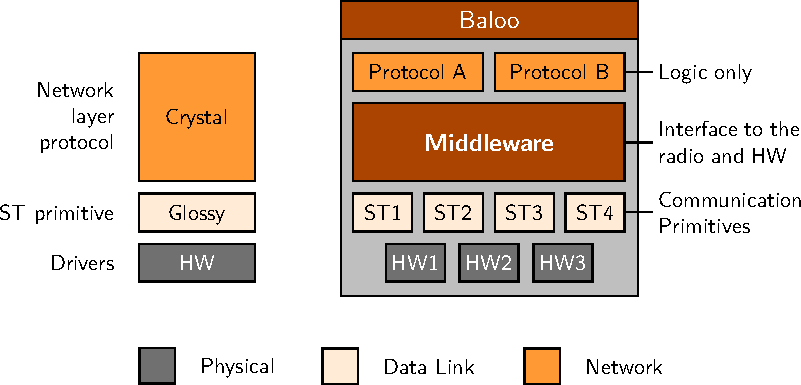
\includegraphics[scale=1]{stack_baloo.pdf}\\~\\
  \begin{minipage}[t]{.47\linewidth}
    \textbf{(a)} The implementation of the network layer protocol (Crystal) couples the interface to the underlying \ST primitive (Glossy) and the protocol logic, \ie how long are the communication rounds, which radio channel is used, \etc
  \end{minipage}
  \hfill
  \begin{minipage}[t]{.47\linewidth}
    \textbf{(b)} Thanks to its additional middleware layer, \baloo flexibly supports multiple \ST primitives and significantly reduces the efforts required to implement  network layer protocols compared to traditional stacks, like LWB~\cite{ferrari2012LWB} or Crystal~\cite{istomin2018Interferenceresilient}.
  \end{minipage}
  %
  \caption{Crystal~\cite{istomin2018Interferenceresilient} is a typical example of network stack based on \ST (\cref{fig:stack_baloo}a).
		Conversely, \baloo is a flexible design framework.
		It is based on a middleware layer that separates the concern of timely execution of \ST primitives from the implementation of the protocol logic (\cref{fig:stack_baloo}b).}
	\label{fig:stack_baloo}
\end{figure}

This chapter \emph{is not} meant to cover all details and inner mechanisms of \baloo, but mainly presents the core concepts of the framework.
\baloo is open source and the complete technical documentation is available online~(\cref{append:baloo_artifacts}).
